% Created 2016-10-25 Tue 11:59
\documentclass[bigger]{beamer}
\usepackage[latin1]{inputenc}
\usepackage[T1]{fontenc}
\usepackage{fixltx2e}
\usepackage{graphicx}
\usepackage{longtable}
\usepackage{float}
\usepackage{wrapfig}
\usepackage{rotating}
\usepackage[normalem]{ulem}
\usepackage{amsmath}
\usepackage{textcomp}
\usepackage{marvosym}
\usepackage{wasysym}
\usepackage{amssymb}
\usepackage{hyperref}
\tolerance=1000
\mode<beamer>{\usetheme{Boadilla}\usecolortheme[RGB={40,100,30}]{structure}}
%\usebackgroundtemplate{\includegraphics[width=\paperwidth]{MNRgreen}}
\setbeamersize{text margin left=10mm}
%\setbeamertemplate{frametitle}{ \vskip20mm \insertframetitle }
\setbeamertemplate{blocks}[rounded][shadow=true]
\graphicspath{{figures/}}
\usetheme{default}
\author{A. Cottrill}
\date{October 25, 2016.}
\title{Untangling UGLMU Gear Codes}
\hypersetup{
  pdfkeywords={},
  pdfsubject={},
  pdfcreator={Emacs 24.5.1 (Org mode 8.2.10)}}
\begin{document}

\maketitle



\begin{frame}[label=sec-1]{Gear}
\begin{itemize}
\item CPUE is the fundamental measure of virtually all fisheries
assessment programs
\item effort (in cpue) is directly dependent on the gear that was used to
obtain the catch.
\item impossible to compare cpue numbers without knowledge of gear.
\end{itemize}
\end{frame}


\begin{frame}[label=sec-2]{Existing Data Sources}
\begin{itemize}
\item Gear codes in UGMLU databases are messy
\begin{itemize}
\item some gear descriptions in FN013 and FN014 tables in Fishnet
archive.  Good for many projects in 1990s, earlier projects sketchy,
latter project non-existent
\item some gear fields in master databases (GR, GRTP, EFF, EFFDST) that
allow us to reconstruct some gears
\end{itemize}
\item Darrel's Gear Spreadsheet
\item Lookup tables on server
\item available documentation on Project Tracker
\end{itemize}
\end{frame}

\begin{frame}[label=sec-3]{Gear and our data model}
\begin{itemize}
\item Gear defines FN122 table:
\begin{itemize}
\item one record per sam for traps and hoops
\item one record for each panel of gill nets
\item can't have records for meshes not in gear
\item ProcVal can check for these if gear is well defined and consistent
across projects
\end{itemize}
\end{itemize}
\end{frame}

\begin{frame}[label=sec-4]{Where are we going?}
\begin{figure}
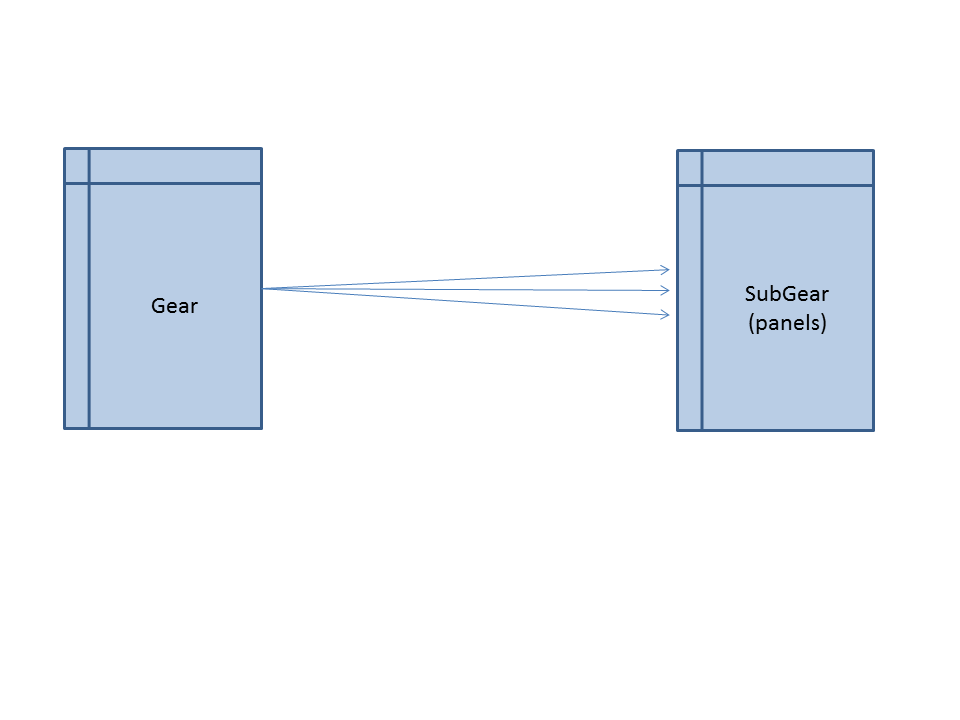
\includegraphics[width=\textwidth]{GearTables1}
\end{figure}
\end{frame}

\begin{frame}[label=sec-5]{Where are we going?}
\begin{figure}
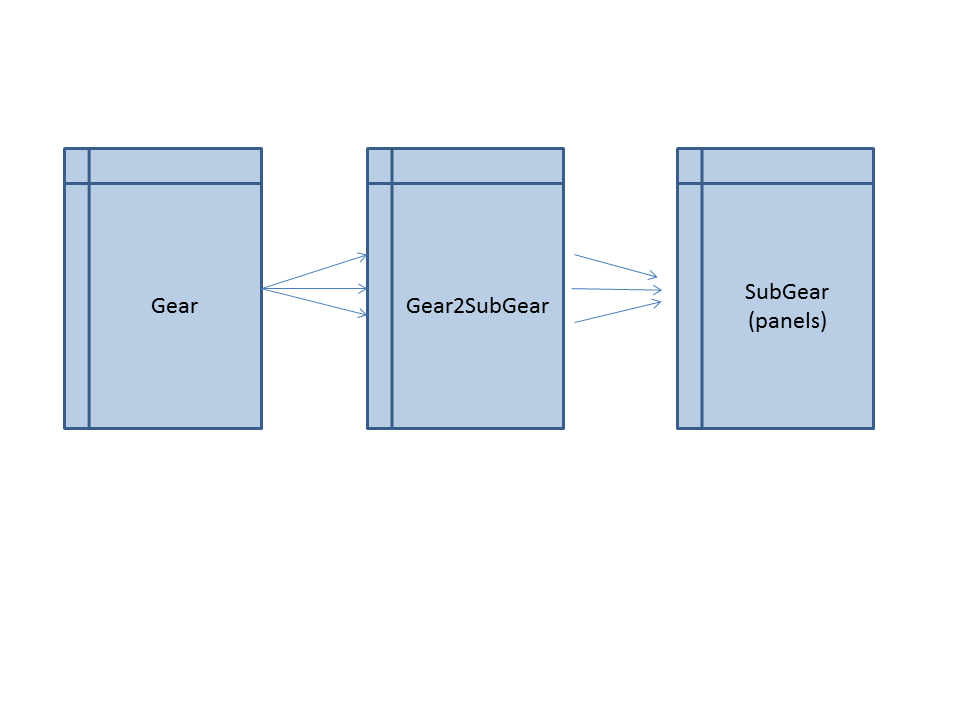
\includegraphics[width=\textwidth]{GearTables2}
\end{figure}
\end{frame}

\begin{frame}[label=sec-6]{Where are we going?}
\begin{figure}
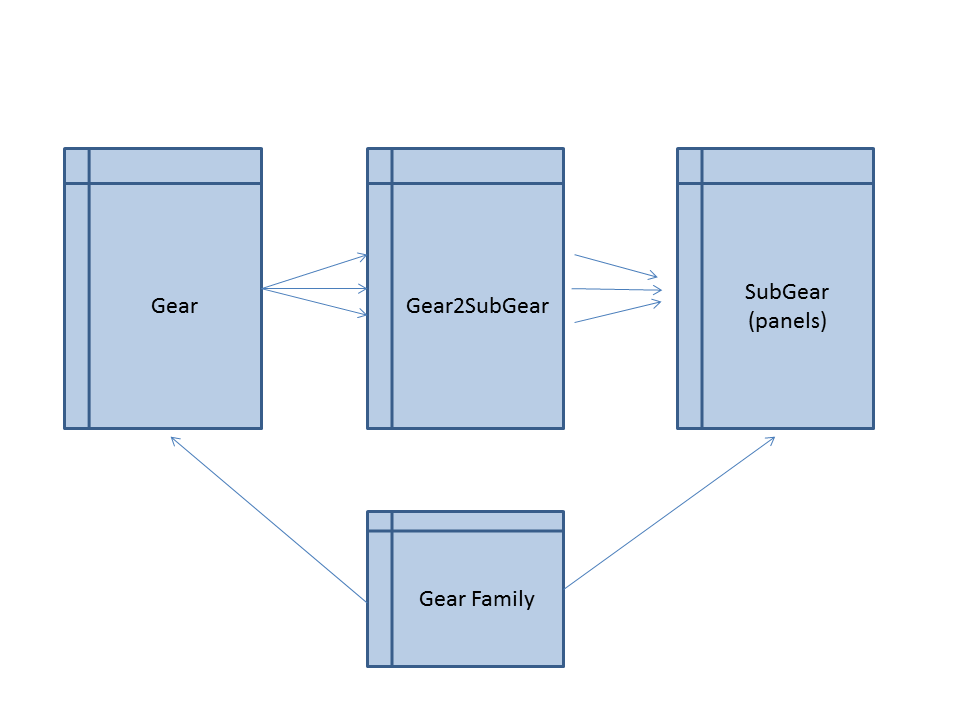
\includegraphics[width=\textwidth]{GearTables3}
\end{figure}
\end{frame}


\begin{frame}[label=sec-7]{Gear:}
\begin{itemize}
\item A master table of gears.  This will evaully replace the FN013
table.
\item Each gear will only be defined once and will be associated
to each SAM by Gear Code (or foreign key).
\end{itemize}
\end{frame}

\begin{frame}[label=sec-8]{Subgear:}
\begin{itemize}
\item A master table of gear panel attributes - each sub-gear will only
be defined once and asscoaited with the appropriate gear through a
many-to-many relationship.
\begin{itemize}
\item For example, the 51mm offshore panel is used in multiple gears,
and each gear has multple panels/subgears.
\end{itemize}
\item analogous to data in Darrel's spreadsheet
\end{itemize}
\end{frame}

\begin{frame}[label=sec-9]{Gear Family:}
\begin{itemize}
\item A table to constrain relationships between gears and sub-gears
\item Gears are comprised of subgears, but only subgears in the same family
should be allowed.
\item For example:

\begin{itemize}
\item GL10, GL21, GL22 and GL32 are all derived from offshore
monofilament (OSIA-mono) panels

\item GL01 is offshore multifilament (OSIA-multi)

\item GL50 is a FWIN family

\item GL38, GL51, GL64 are all part of the FLIN/SLIN family
\end{itemize}
\end{itemize}
\end{frame}

\begin{frame}[label=sec-10]{Gear Family (cont'd):}
\begin{itemize}
\item More Families:
\begin{itemize}
\item Nordic nets
\item Bottle traps
\item GEE traps
\item Windermere traps
\item Smallfish-tall
\item Smallfish-short
\item North American Standard
\item Trap nets
\item Hoop nets
\item Unknown*
\end{itemize}
\end{itemize}
\end{frame}


\begin{frame}[label=sec-11]{Gear2SubGear}
\begin{itemize}
\item association table to facilitate many-to-many between gear and
subgear
\item contains additional information:
\begin{itemize}
\item panel sequence
\item panel count
\end{itemize}
\end{itemize}
\end{frame}

\begin{frame}[label=sec-12]{How we are going to get there?}
\begin{itemize}
\item use fn\_portal
\item database tables for old fishnet tables have been created and populated
\begin{itemize}
\item tables from the fish net archive will be used where possible
\item more recent data will be populated from gear codes where gear
details are known (e.g. - offshore gears)
\item project leads, field staff may be asked to provide some input
\end{itemize}

\item Gear, subgear and gear family tables have been created and populated
from available data.

\item summary of gears used in a project have been be added to project details
in fn\_portal
\end{itemize}
\end{frame}

\begin{frame}[label=sec-13]{How we are going to get there?}
\begin{itemize}
\item views have been created in fn\_portal to:
\begin{itemize}
\item list gears
\item gear details
\begin{itemize}
\item about the gear
\item associated sub-gears
\item projects where gear was used
\item active/depreciated
\item confirmed
\end{itemize}
\item edit gear description
\end{itemize}
\item list of gears to be updated by <USER>
\end{itemize}
\end{frame}

\begin{frame}[label=sec-14]{What have we learned?}
\begin{itemize}
\item all projects need specific project protocols (many are missing from
project tracker)
\item project protocols need to explicit describe gear used in project
\begin{itemize}
\item generic "same as other project" shortcuts are not adequate
\end{itemize}
\item science 101 - sufficient detail to reproduce/re-run project
\end{itemize}
\end{frame}

\begin{frame}[label=sec-15]{Gill Net Examples}
\begin{figure}
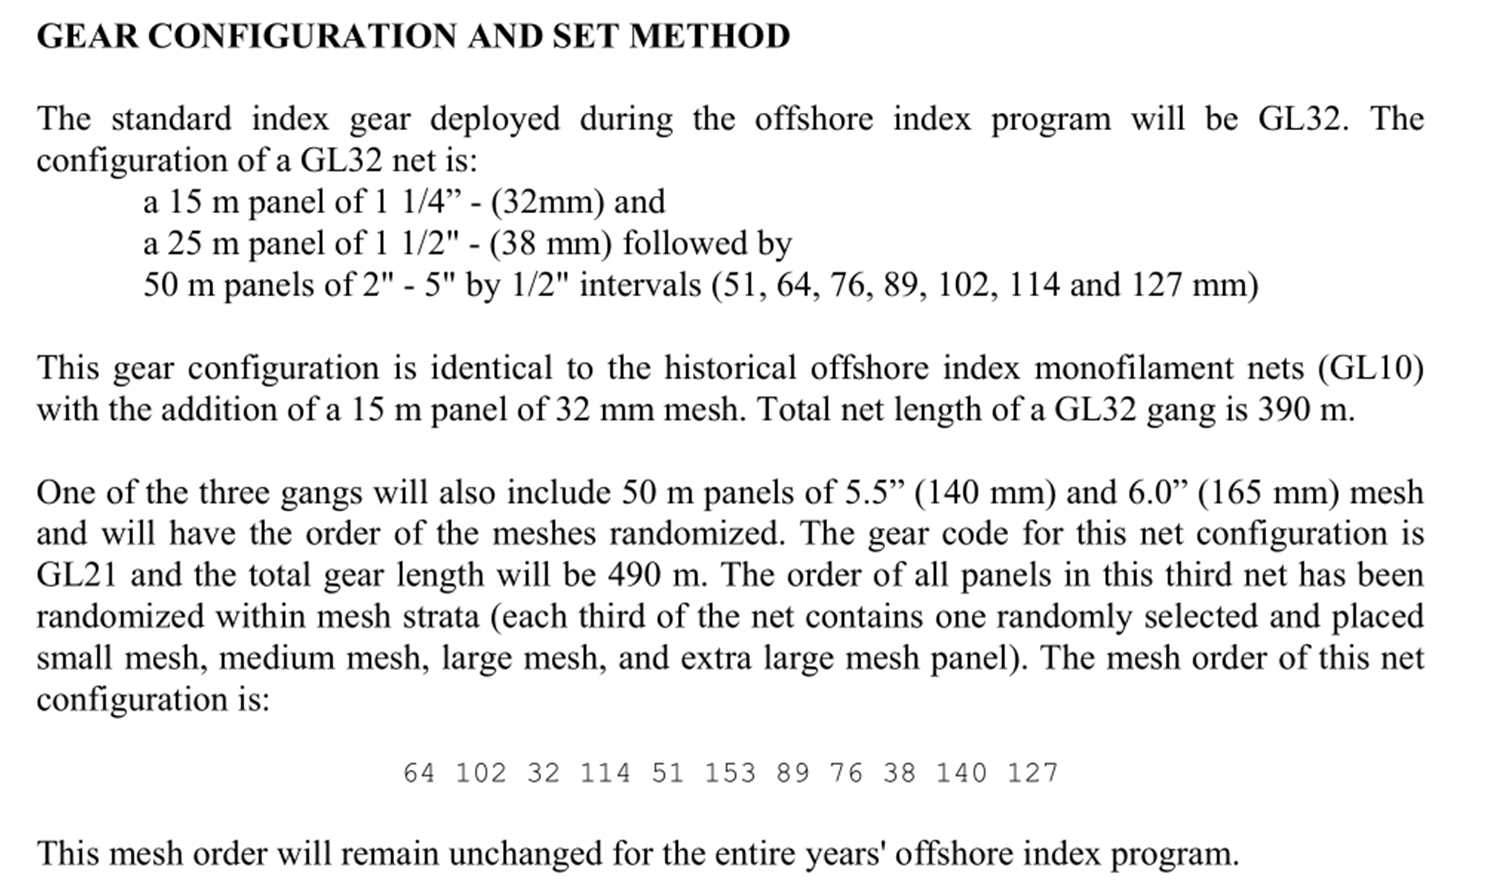
\includegraphics[width=\textwidth]{GN_Example}
\end{figure}
\end{frame}

\begin{frame}[label=sec-16]{Trap Net Examples}
\begin{figure}
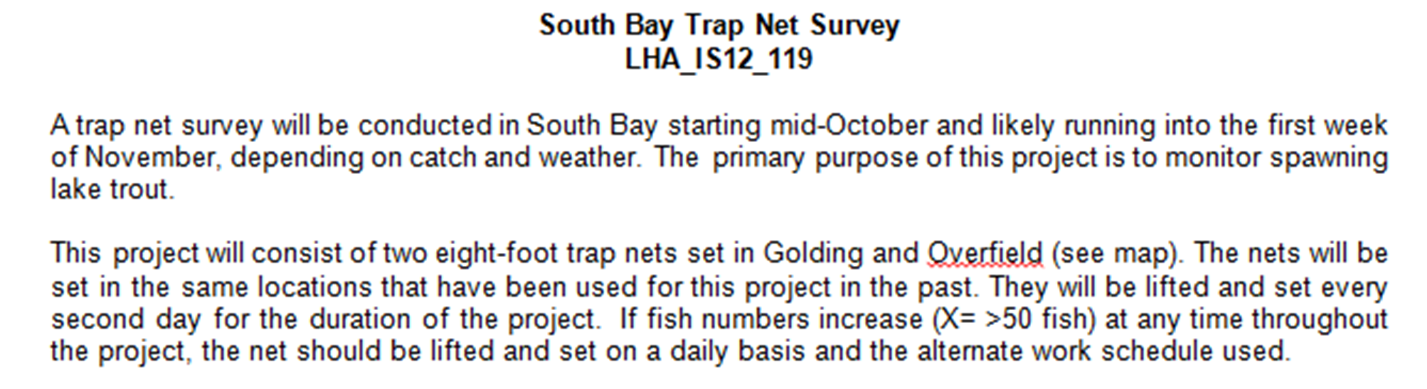
\includegraphics[width=\textwidth]{TP_Example}
\end{figure}
\end{frame}


\begin{frame}[label=sec-17]{Other Gears:}
\begin{itemize}
\item any suggestions?
\begin{itemize}
\item fyke nets
\item hoop nets
\item bottle traps
\item Windermere traps
\item electrofishing
\item others\ldots{}
\end{itemize}
\end{itemize}
\end{frame}

\begin{frame}[label=sec-18]{Consolidating Gear codes}
\begin{itemize}
\item process of updating project masters to match gear master
\item documenting undocumented GL and TP codes
\begin{itemize}
\item inspecting FN122, FN123 and FN125 tables.  Inferring gear from
similar projects in same year
\end{itemize}
\item FishNet Archive/FishLib
\begin{itemize}
\item possible our archive are incomplete,  especially for projects run
by other offices (Espanola/Severn Sound)
\end{itemize}
\end{itemize}
\end{frame}

\begin{frame}[label=sec-19]{Trap Nets}
\begin{itemize}
\item 3 proposed codes:
\begin{itemize}
\item TP06 - Standard 6' trap net
\item TP08 - Standard 8' trap net
\item TP  - Undocumented trap net (only in rare cases)
\end{itemize}
\item update masters to these codes where information exists to identify
trap net size
\end{itemize}
\end{frame}

\begin{frame}[label=sec-20]{Gill Nets}
\begin{itemize}
\item eliminate gear code synonyms
\item update gear codes where inconsistencies are evident
\end{itemize}
\end{frame}


\begin{frame}[label=sec-21]{Next Steps/Homework}
\begin{itemize}
\item confirm assigned gears:
\begin{itemize}
\item provide description for assigned gear
\item verify sub gear attributes:
\begin{itemize}
\item populate where possible
\item check existing values
\end{itemize}
\end{itemize}
\item FLIN gear used with one or multiple efforts. Can these be the same gear
code?
\begin{itemize}
\item 1 can mean half of the net or all of the net
\end{itemize}
\item export gear code master tables
\item update proc-val to query master tables
\end{itemize}
\end{frame}
% Emacs 24.5.1 (Org mode 8.2.10)
\end{document}
